\chapter{Estrategia de Implementaci\'on y An\'alisis de Resultados}

\section{Estrategia y Entorno de Implementaci\'on}

El desarrollo computacional del proyecto se articul\'o en una arquitectura h\'ibrida que desacopla la fase de entrenamiento a gran escala en la nube (\textit{Cloud Training}) de la fase de operaci\'on local en el tel\'efono (\textit{Edge Inference}).

\subsection{Infraestructura de C\'omputo y Entrenamiento en la Nube}
Los modelos se entrenaron sobre instancias aceleradas por hardware en la plataforma Modal, empleando unidades de procesamiento gr\'afico \textbf{NVIDIA A10G} (24~GB VRAM GDDR6, 125 TFLOPS de rendimiento tensorial) montadas sobre entornos Linux con CUDA 12.1 y PyTorch 2.3. Se aplic\'o precisi\'on mixta autom\'atica (\textit{AMP bfloat16}) para maximizar el ancho de banda y la saturaci\'on de memoria.

El r\'egimen de entrenamiento incorpor\'o un programador de tasa de aprendizaje por recocido cosenoidal con calentamiento lineal (\textit{Cosine Annealing with Warmup}) durante tres \'epocas iniciales, estabilizando los pesos procedentes de ImageNet antes de permitir gradientes elevados. Como salvaguarda frente al sobreajuste, se aplic\'o parada temprana (\textit{Early Stopping}) con una paciencia de 8 \'epocas sobre el Macro $F_1$ de validaci\'on (Figura~\ref{fig:convergencia_entrenamiento}).

\begin{figure}[H]
\centering
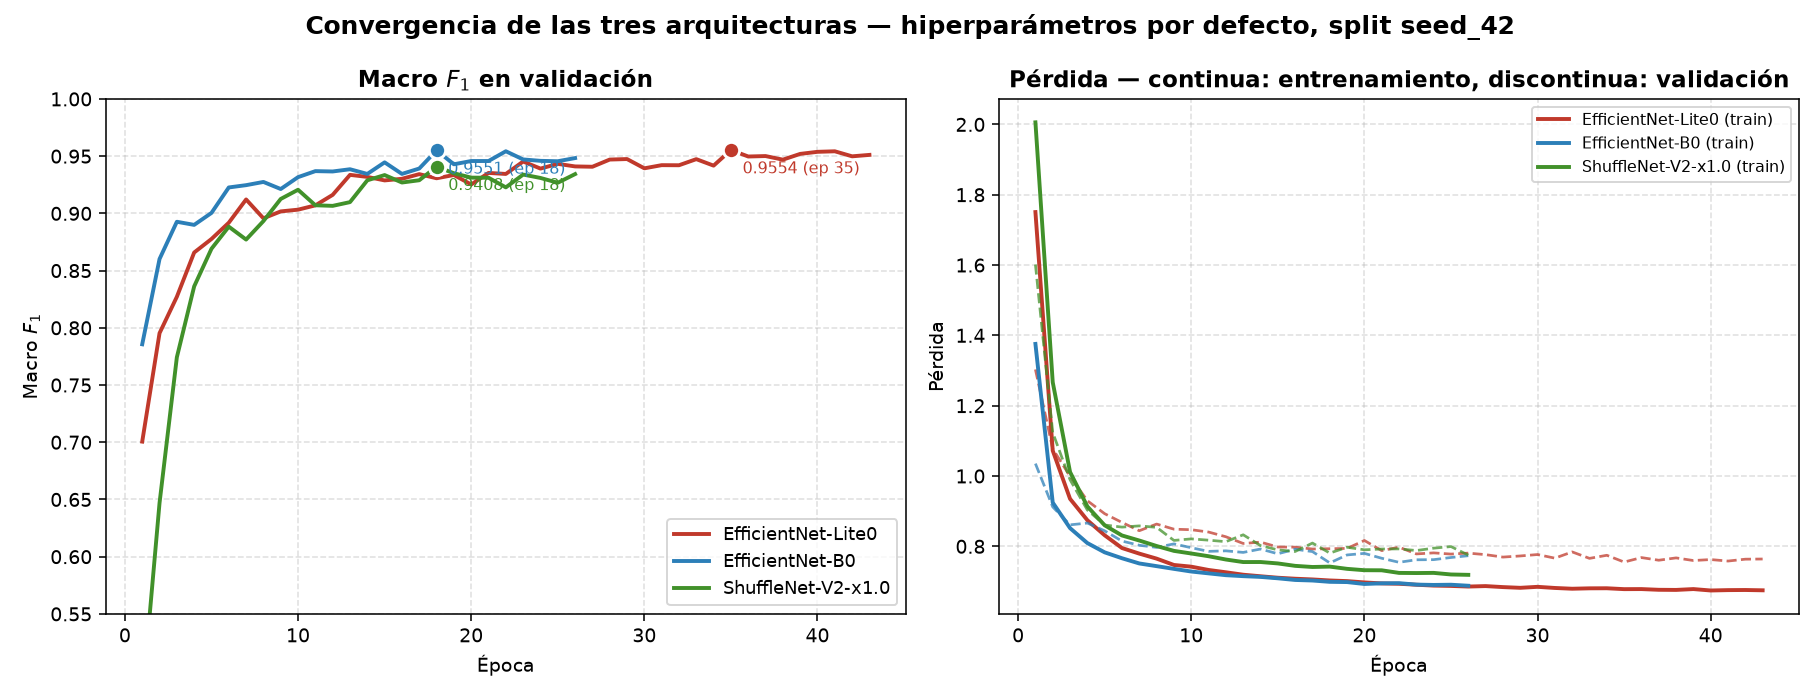
\includegraphics[width=0.78\linewidth]{images/training/training_convergence.png}
\caption{Curvas de convergencia: P\'erdida y Macro $F_1$ durante el entrenamiento en Modal.}
\label{fig:convergencia_entrenamiento}
\end{figure}

\section{Resultados por Tema de Evaluaci\'on}

Los resultados se agrupan en los cuatro temas de los criterios de \'exito (Tabla~\ref{tab:criterios_exito}). Cada subsecci\'on reporta solo valores medidos y, cuando el criterio no se cumple o no se midi\'o, lo indica.

\subsection{Ahorro de entrenamiento: b\'usqueda bayesiana con poda}

El estudio bayesiano ejecutado con Optuna explor\'o 25 intentos sobre la arquitectura \texttt{EfficientNet-Lite0}, de los cuales 8 se completaron, 15 fueron podados por el algoritmo \textit{MedianPruner} al no superar la mediana de sus pares tras el periodo de calentamiento (8 \'epocas), y 2 se interrumpieron por fallos de proceso. El ensayo ganador fue el Trial~0 (\'epoca 44), seleccionado por su mejor Macro $F_1$ de validaci\'on.

\begin{figure}[H]
\centering
\begin{minipage}[b]{0.48\linewidth}
\centering
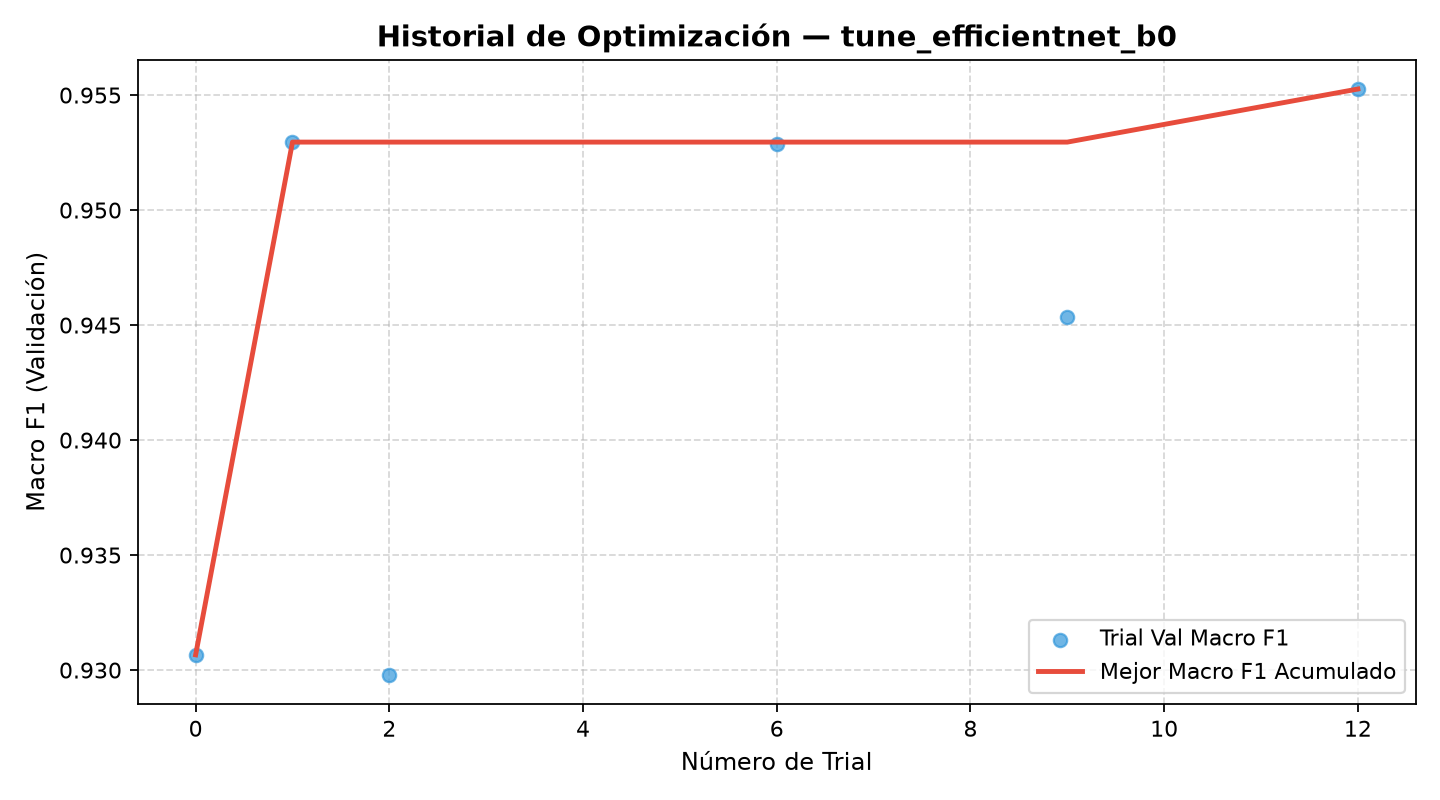
\includegraphics[width=\linewidth]{images/tuning/optimization_history.png}
\caption{Historial de ensayos de Optuna.}
\label{fig:opt_hist}
\end{minipage}
\hfill
\begin{minipage}[b]{0.48\linewidth}
\centering
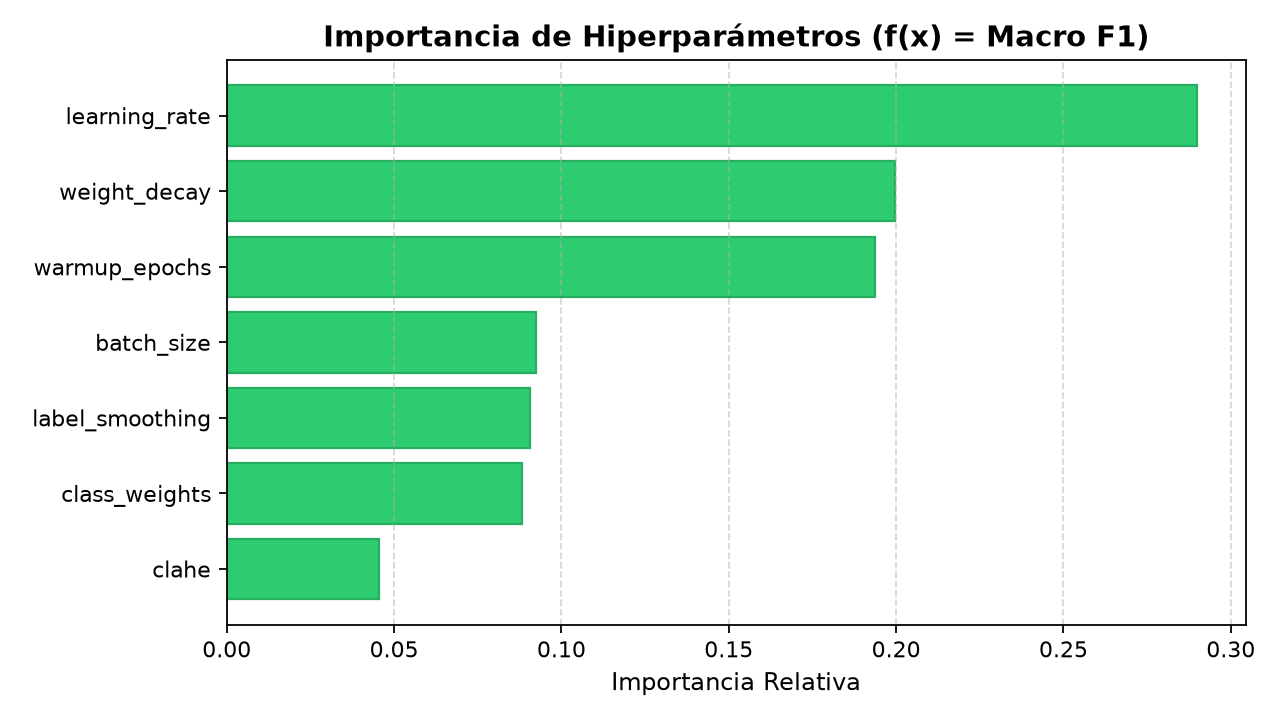
\includegraphics[width=\linewidth]{images/tuning/param_importances.png}
\caption{Importancia relativa de hiperpar\'ametros.}
\label{fig:param_imp}
\end{minipage}
\caption{Din\'amica de exploraci\'on e impacto relativo de variables en Optuna.}
\end{figure}

El an\'alisis de importancia (Figura~\ref{fig:param_imp}) revel\'o que el calentamiento (\texttt{warmup\_epochs}, 0.52), la ponderaci\'on de p\'erdida (\texttt{class\_weights}, 0.15), el suavizado de etiquetas (\texttt{label\_smoothing}, 0.11), la tasa de aprendizaje (\texttt{learning\_rate}, 0.10) y el tama\~no de lote (\texttt{batch\_size}, 0.09) concentran la mayor parte de la variaci\'on del objetivo. La configuraci\'on del Trial~0 comparada con la l\'inea base se muestra en la Tabla~\ref{tab:opt_vs_base_c3}.

\begin{table}[H]
\caption{Comparativa cuantitativa: Baseline sin Optuna vs. Configuraci\'on Optimizada (Optuna)}
\label{tab:opt_vs_base_c3}
\centering
\small
\begin{singlespace}
\begin{tabular}{lccc}
\toprule
\textbf{M\'etrica / Variable} & \textbf{Sin Optuna (Base)} & \textbf{Optimizada (Optuna)} & \textbf{Impacto / Delta} \\
\midrule
Macro $F_1$ en Validaci\'on & 0.9561 & 0.9573 & +0.12 pp \\
\textbf{Macro $F_1$ en Prueba Retenida} & 0.9480 & 0.9431 & $-0.49$ pp \\
Tasa de Aprendizaje (\texttt{lr}) & $1.00 \times 10^{-4}$ & $8.47 \times 10^{-5}$ & Valor de b\'usqueda \\
Tama\~no de Lote (\texttt{batch\_size}) & 32 & 16 & Valor de b\'usqueda \\
Ponderaci\'on de P\'erdida & \texttt{sqrt\_inverse} & \texttt{none} & Valor de b\'usqueda \\
Suavizado de Etiquetas & 0.10 & 0.075 & Valor de b\'usqueda \\
\bottomrule
\end{tabular}
\end{singlespace}
\end{table}

\noindent\textbf{Resultado de prueba y decisi\'on de configuraci\'on:} El ensayo ganador no mejor\'o el Macro $F_1$ de prueba frente a la l\'inea base ($-0.49$ pp), aunque s\'i mejor\'o ligeramente la validaci\'on (+0.12 pp). Por ese motivo, el ganador no se utiliz\'o para reemplazar la configuraci\'on de desarrollo, que es la de la ejecuci\'on \texttt{20260921\_204608} (\texttt{learning\_rate} $10^{-4}$, lote 32, \texttt{sqrt\_inverse}, suavizado 0.1), con Macro $F_1$ de prueba de \textbf{0.9480} y exactitud de 97.81\%. Esta ejecuci\'on es la oficial del proyecto por ser la m\'as reciente y completa. El presupuesto de b\'usqueda se redujo de 60 a 25 intentos despu\'es de observar resultados parciales, mediante una enmienda registrada.

\subsection{Rendimiento del modelo: ensamble y bioseguridad}

El ensamble heterog\'eneo por votaci\'on suave (\textit{Soft Voting}) super\'o a todas las arquitecturas individuales en la totalidad de las m\'etricas de evaluaci\'on (Tabla~\ref{tab:resultados_ensamble_c3} y Figura~\ref{fig:comparativa_ensamble_bar}).

\begin{table}[H]
\caption{Desempe\~no cuantitativo del Ensamble vs. Modelos Individuales en Prueba (5~015 im\'agenes)}
\label{tab:resultados_ensamble_c3}
\centering
\small
\begin{singlespace}
\begin{tabular}{lcccc}
\toprule
\textbf{Arquitectura / Modelo} & \textbf{Exactitud (Accuracy)} & \textbf{Macro $F_1$} & \textbf{Precision} & \textbf{Recall} \\
\midrule
ShuffleNet-V2-x1.0 & 97.31\% & 0.9330 & 0.9388 & 0.9298 \\
EfficientNet-Lite0 (Referencia oficial, base de desarrollo) & 97.81\% & 0.9480 & 0.9513 & 0.9467 \\
EfficientNet-B0 (Referencia Individual) & 97.97\% & 0.9483 & 0.9589 & 0.9400 \\
\textbf{Ensamble Heterog\'eneo (Soft Voting)} & \textbf{98.29\%} & \textbf{0.9567} & \textbf{0.9642} & \textbf{0.9506} \\
\midrule
\textit{Ganancia neta vs. Mejor Individual} & \textit{+0.32 pp} & \textit{+0.84 pp} & \textit{+0.53 pp} & \textbf{\textit{+1.06 pp}} \\
\bottomrule
\end{tabular}
\end{singlespace}
\end{table}

\begin{figure}[H]
\centering
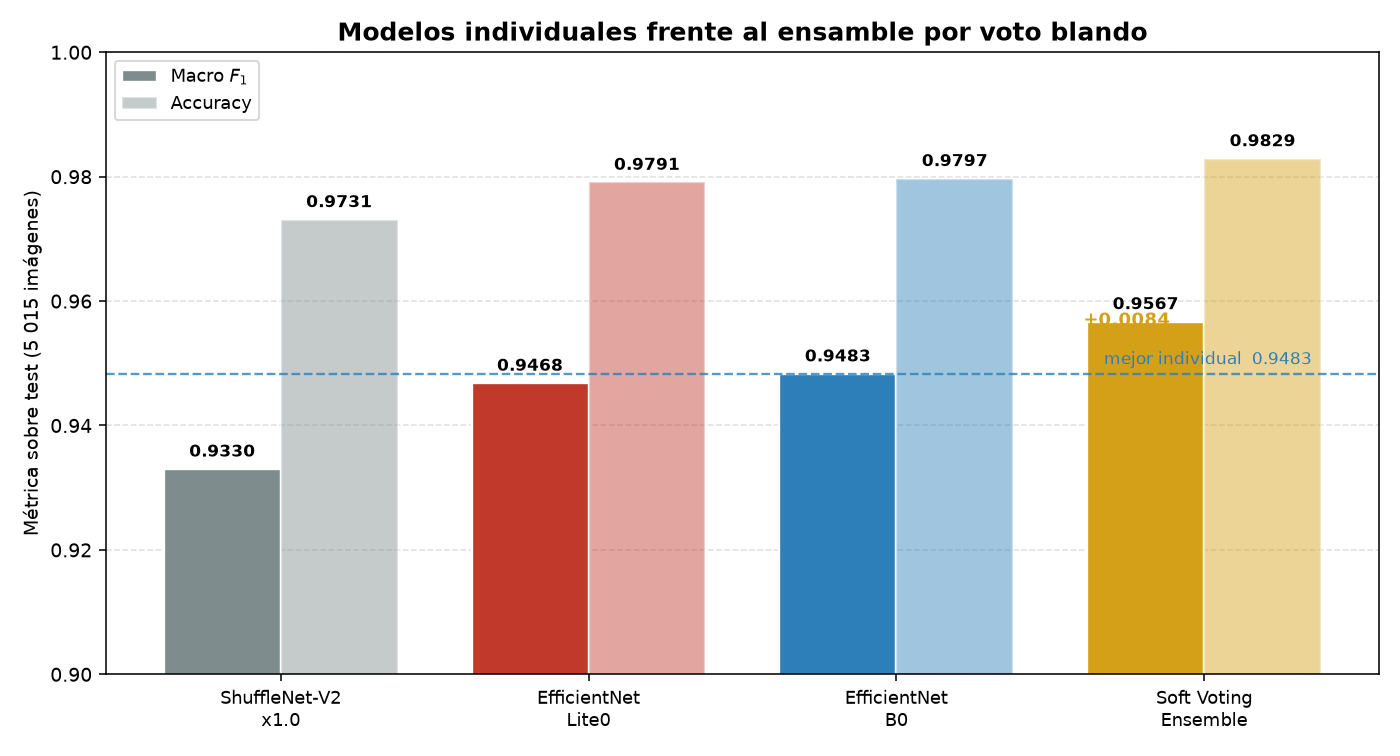
\includegraphics[width=0.72\linewidth]{images/ensemble/ensemble_comparison_bar.png}
\caption{Comparativa de desempe\~no del ensamble frente a modelos individuales.}
\label{fig:comparativa_ensamble_bar}
\end{figure}

El hallazgo de mayor trascendencia agron\'omica reside en el \textbf{Macro Recall de 95.06\%}. En fitopatolog\'ia, el costo de un falso negativo es devastador: omitir una infecci\'on incipiente permite que el hongo o virus arrase con la parcela. Como lo demuestra la matriz de confusi\'on normalizada del ensamble (Figura~\ref{fig:matriz_ensamble}), la \textbf{Necrosis Letal del Ma\'iz (MLN)} alcanz\'o un \textbf{Recall perfecto del 100.0\% (963 aciertos sobre 963 casos de prueba, cero falsos negativos)}. La roya com\'un y el tiz\'on superaron el 98\% de detecci\'on.

\begin{figure}[H]
\centering
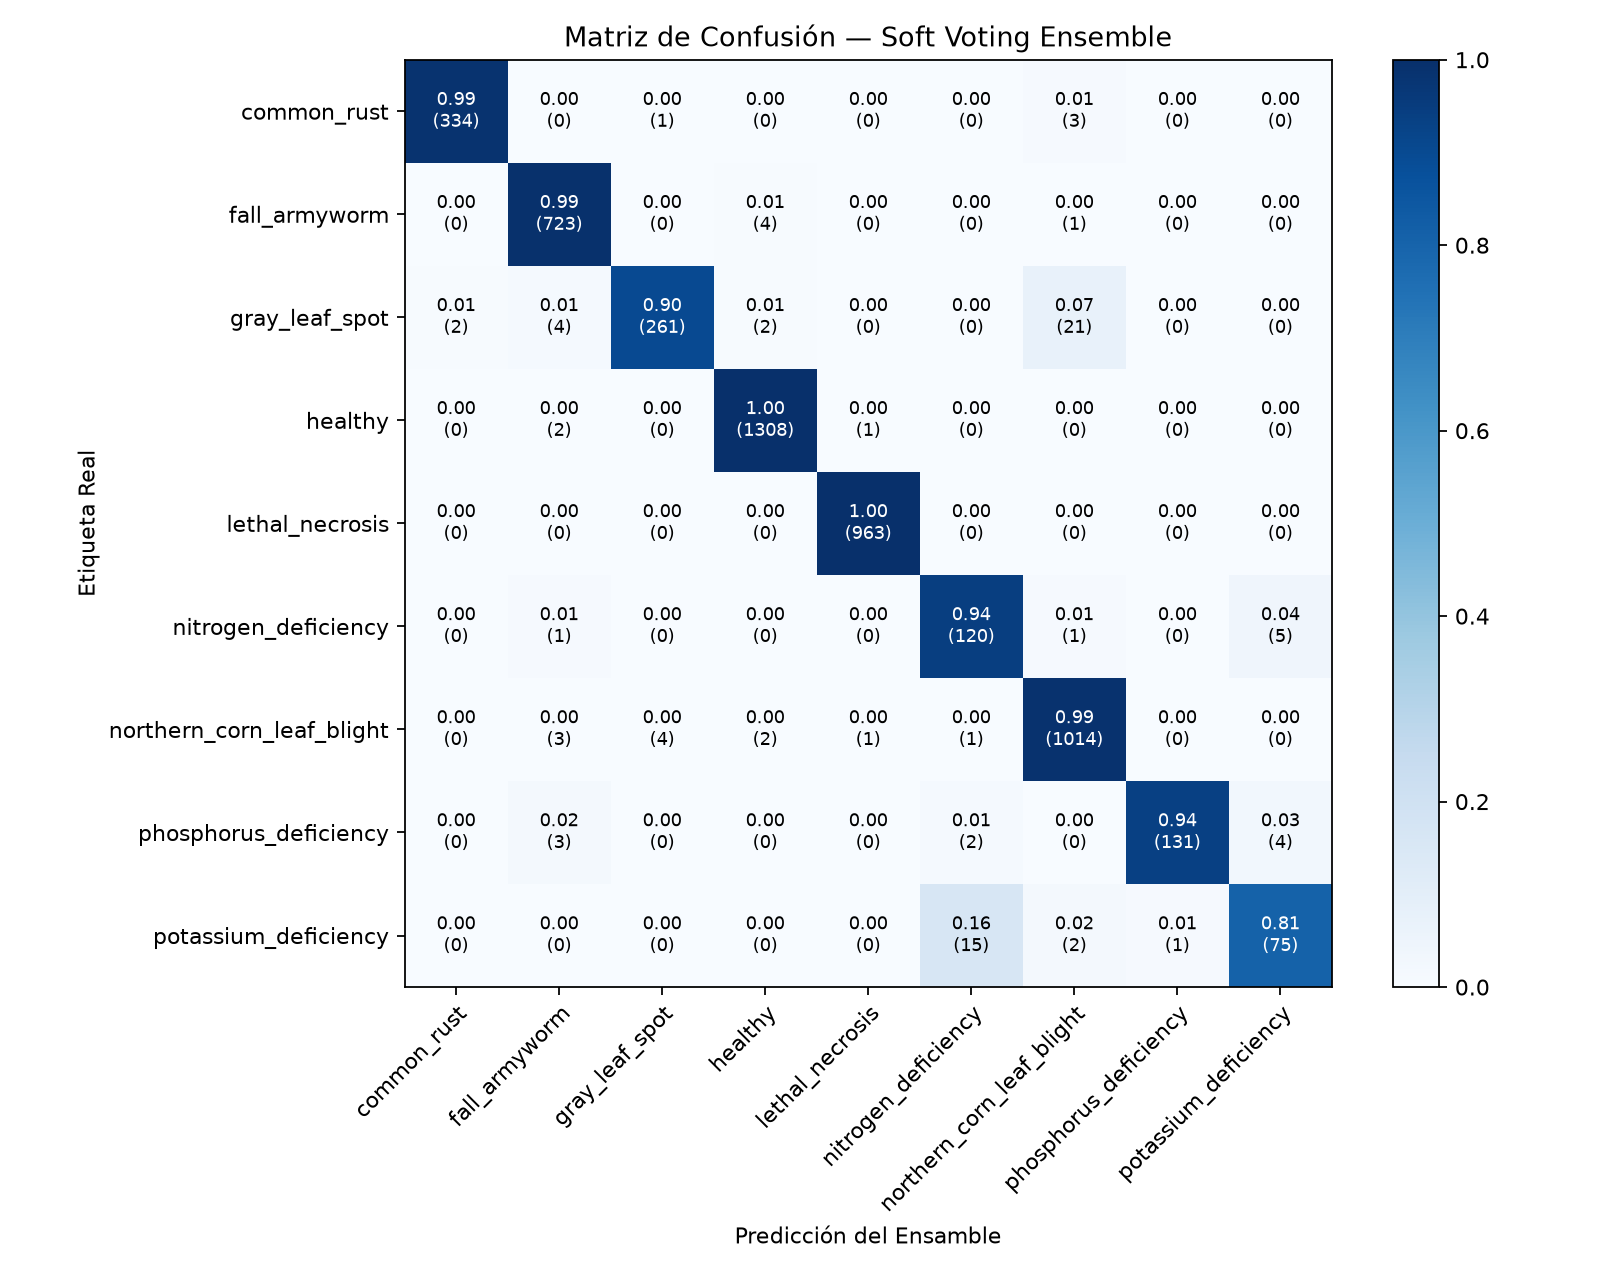
\includegraphics[width=0.68\linewidth]{images/ensemble/confusion_matrix_ensemble.png}
\caption{Matriz de confusi\'on normalizada del ensamble sobre 5~015 muestras de prueba.}
\label{fig:matriz_ensamble}
\end{figure}

Asimismo, se resolvi\'o definitivamente el cuello de botella hist\'orico de la primera fase: la \textbf{deficiencia de potasio}, que previamente colapsaba en 0.49, ascendi\'o a \textbf{0.8475} en el ensamble y a 0.8242 en Lite0. Esta mejora coincide con la incorporaci\'on de nuevos repositorios y con la p\'erdida ponderada \texttt{sqrt\_inverse}, pero no se aisl\'o experimentalmente la contribuci\'on de cada factor.

\begin{table}[H]
\caption{Desglose de rendimiento agron\'omico por clase en el conjunto de prueba independiente}
\label{tab:desglose_clases}
\centering
\small
\begin{singlespace}
\begin{tabular}{lccccc}
\toprule
\textbf{Patolog\'ia Agron\'omica} & \textbf{Soporte} & \textbf{Lite0 ($F_1$)} & \textbf{B0 ($F_1$)} & \textbf{ShuffleNet ($F_1$)} & \textbf{Ensamble ($F_1$)} \\
\midrule
Necrosis Letal (MLN) & 963 & 0.9964 & 0.9984 & 0.9974 & \textbf{0.9990} \\
Planta Sana (Healthy) & 1~311 & 0.9924 & 0.9954 & 0.9901 & \textbf{0.9958} \\
Roya Com\'un & 339 & 0.9882 & 0.9896 & 0.9867 & \textbf{0.9911} \\
Gusano Cogollero & 728 & 0.9843 & 0.9877 & 0.9815 & \textbf{0.9877} \\
Tiz\'on Foliar (NCLB) & 1~025 & 0.9766 & 0.9769 & 0.9728 & \textbf{0.9811} \\
Mancha Gris (GLS) & 289 & \textbf{0.9331} & 0.9194 & 0.9120 & 0.9388 \\
Deficiencia de F\'osforo & 140 & 0.9318 & 0.9527 & 0.9275 & \textbf{0.9632} \\
Deficiencia de Nitr\'ogeno & 127 & 0.9051 & 0.8939 & 0.8613 & \textbf{0.9057} \\
Deficiencia de Potasio & 93 & 0.8242 & 0.8208 & 0.7674 & \textbf{0.8475} \\
\midrule
\textbf{Macro Promedio} & \textbf{5~015} & \textbf{0.9480} & \textbf{0.9483} & \textbf{0.9330} & \textbf{0.9567} \\
\bottomrule
\end{tabular}
\end{singlespace}
\end{table}

\subsection{Rendimiento del modelo: generalizaci\'on entre fuentes}

Para poner a prueba los l\'imites del sistema frente al cambio de dominio, se dise\~n\'o un experimento cruzado $2\times2$ de validaci\'on cruzada en 5 pliegues sobre \texttt{EfficientNet-Lite0}, comparando la partici\'on estratificada habitual frente a una partici\'on agrupada por procedencia que veta cualquier solapamiento de fuentes entre entrenamiento y evaluaci\'on (Tabla~\ref{tab:kfold_2x2_c3} y Figura~\ref{fig:kfold_2x2_grafico}).

\begin{table}[H]
\caption{Resultados del experimento cruzado $2\times2$ de validaci\'on cruzada en 5 pliegues}
\label{tab:kfold_2x2_c3}
\centering
\small
\begin{singlespace}
\begin{tabular}{lccc}
\toprule
\textbf{Configuraci\'on de Red} & \textbf{CV Estratificada (5 folds)} & \textbf{CV Agrupada por Fuente} & \textbf{Ca\'ida Neta ($\Delta$)} \\
\midrule
Configuraci\'on Base & $0.9311 \pm 0.0099$ & $\mathbf{0.6026 \pm 0.1240}$ & $\mathbf{-0.3286}$ \\
Configuraci\'on B0 & $0.9463 \pm 0.0052$ & $0.6499 \pm 0.1508$ & $-0.2964$ \\
\midrule
\textit{Fuentes en Validaci\'on} & \textit{11 de 11 (100\% solapadas)} & \textit{0 solapadas con entrenamiento} & — \\
\bottomrule
\end{tabular}
\end{singlespace}
\end{table}

\begin{figure}[H]
\centering
\begin{minipage}[b]{0.48\linewidth}
\centering
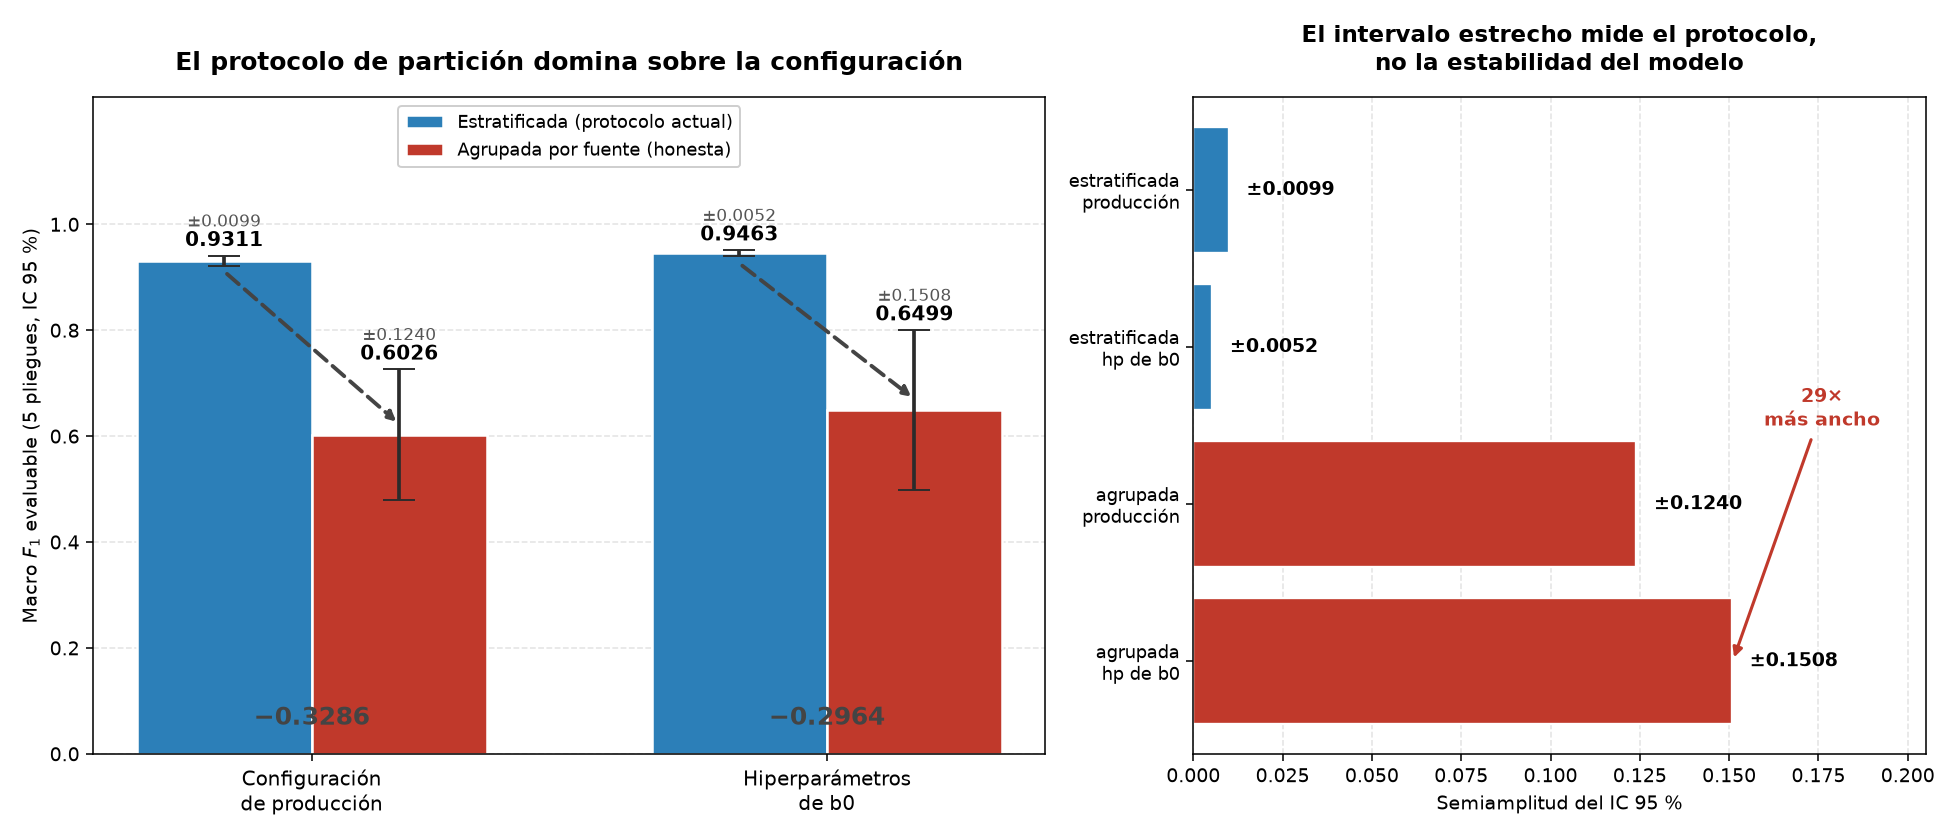
\includegraphics[width=\linewidth]{images/resultados/kfold_2x2.png}
\caption{Dise\~no del experimento cruzado $2\times2$.}
\label{fig:kfold_2x2_grafico}
\end{minipage}
\hfill
\begin{minipage}[b]{0.48\linewidth}
\centering
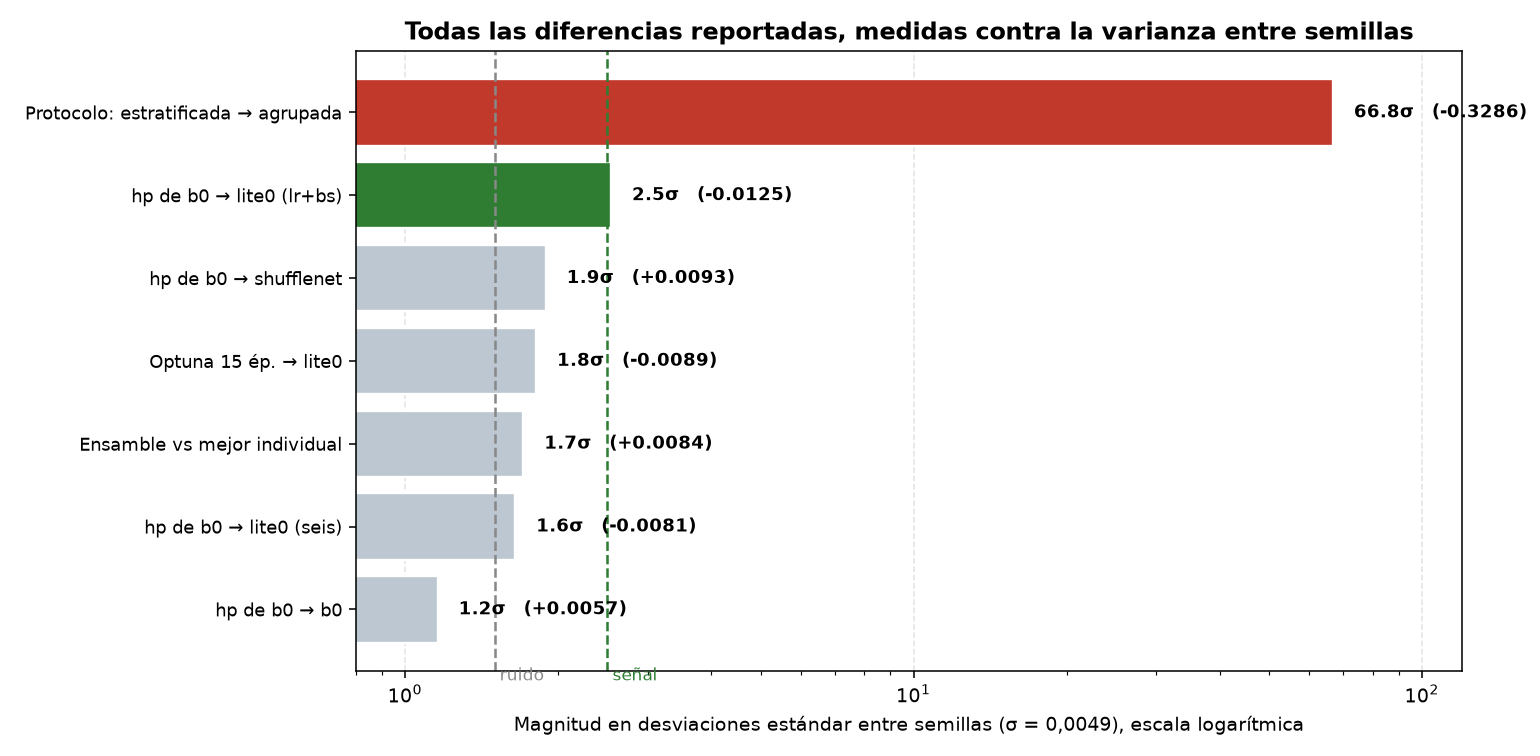
\includegraphics[width=\linewidth]{images/resultados/diferencias_en_sigmas.png}
\caption{Magnitud de impacto en sigmas ($\sigma$).}
\label{fig:sigmas_c3}
\end{minipage}
\caption{Impacto de la partici\'on frente a la optimizaci\'on algor\'itmica.}
\end{figure}

\noindent\textbf{Hallazgo principal:} \textbf{El cambio de protocolo de partici\'on ($-0.3286$ en Macro $F_1$) es considerablemente mayor que el efecto medido del ajuste de hiperpar\'ametros ($+0.0012$ en validaci\'on)}. Mientras la validaci\'on estratificada muestra un intervalo estrecho ($\pm 0.0099$), al evaluar fuera de fuente el Macro $F_1$ baja a $0.6026 \pm 0.1240$, calculado sobre las clases evaluables en cada pliegue.

La variabilidad entre tres semillas en la configuraci\'on oficial es de $\sigma = 0.0049$ (media $0.9430$), por lo que la diferencia de partici\'on equivale a unas 60 desviaciones est\'andar (Figura~\ref{fig:sigmas_c3}). Este resultado es consistente con que las redes entrenadas sobre estos repositorios p\'ublicos dependen en parte de la firma visual de cada fuente, aunque el experimento no permite atribuir la ca\'ida a un \'unico factor.

\subsection{Capacidades del diagn\'ostico: equidad entre entornos}

Se audit\'o el modelo desplegado (\texttt{Lite0}) desglosando la prueba entre im\'agenes en condiciones de laboratorio ($N=532$) y campo aut\'entico ($N=4~483$). En las tres clases compartidas (roya, mancha gris y tiz\'on), el \textit{Disparate Impact Ratio} sobre Macro $F_1$ fue $DIR = 0.9778$ (diferencia de 0.0209), por encima del umbral regulatorio del 80\% (Figura~\ref{fig:fairness_panel}). El umbral mide la paridad de resultados entre grupos y no sustituye el an\'alisis de tasas de error por clase, que se presenta a continuaci\'on.

\begin{figure}[H]
\centering
\begin{minipage}[b]{0.48\linewidth}
\centering
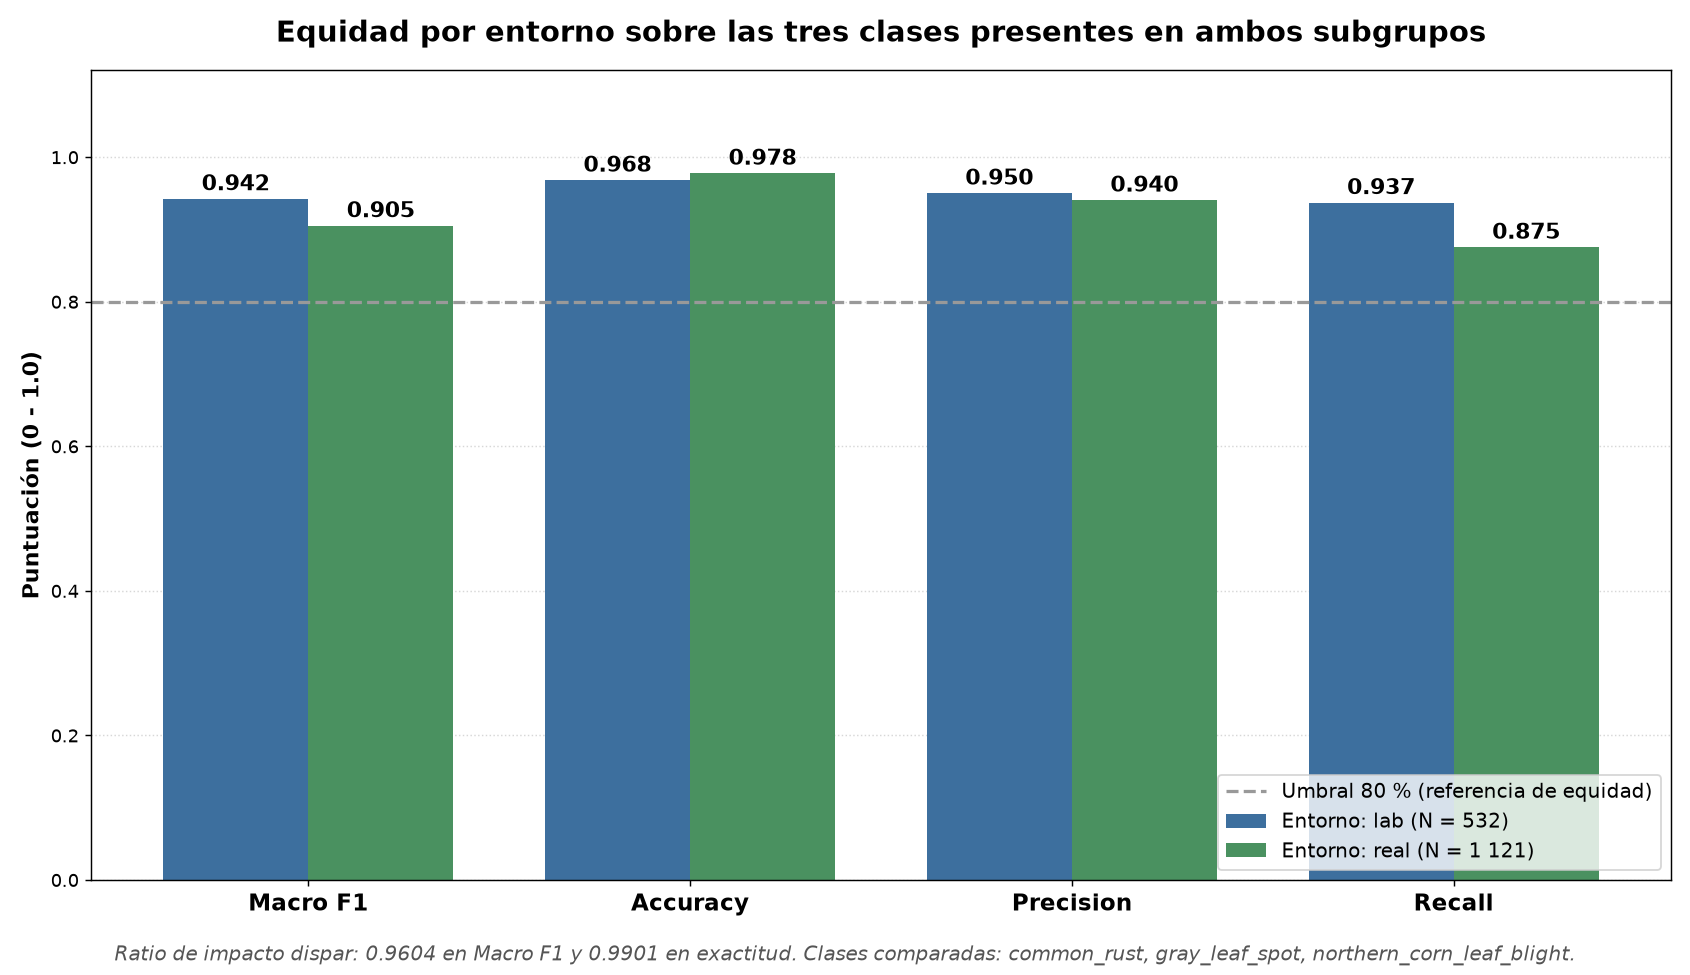
\includegraphics[width=\linewidth]{images/fairness/fairness_disparity.png}
\caption{Disparidad por entorno ambiental.}
\label{fig:fairness_disp}
\end{minipage}
\hfill
\begin{minipage}[b]{0.48\linewidth}
\centering
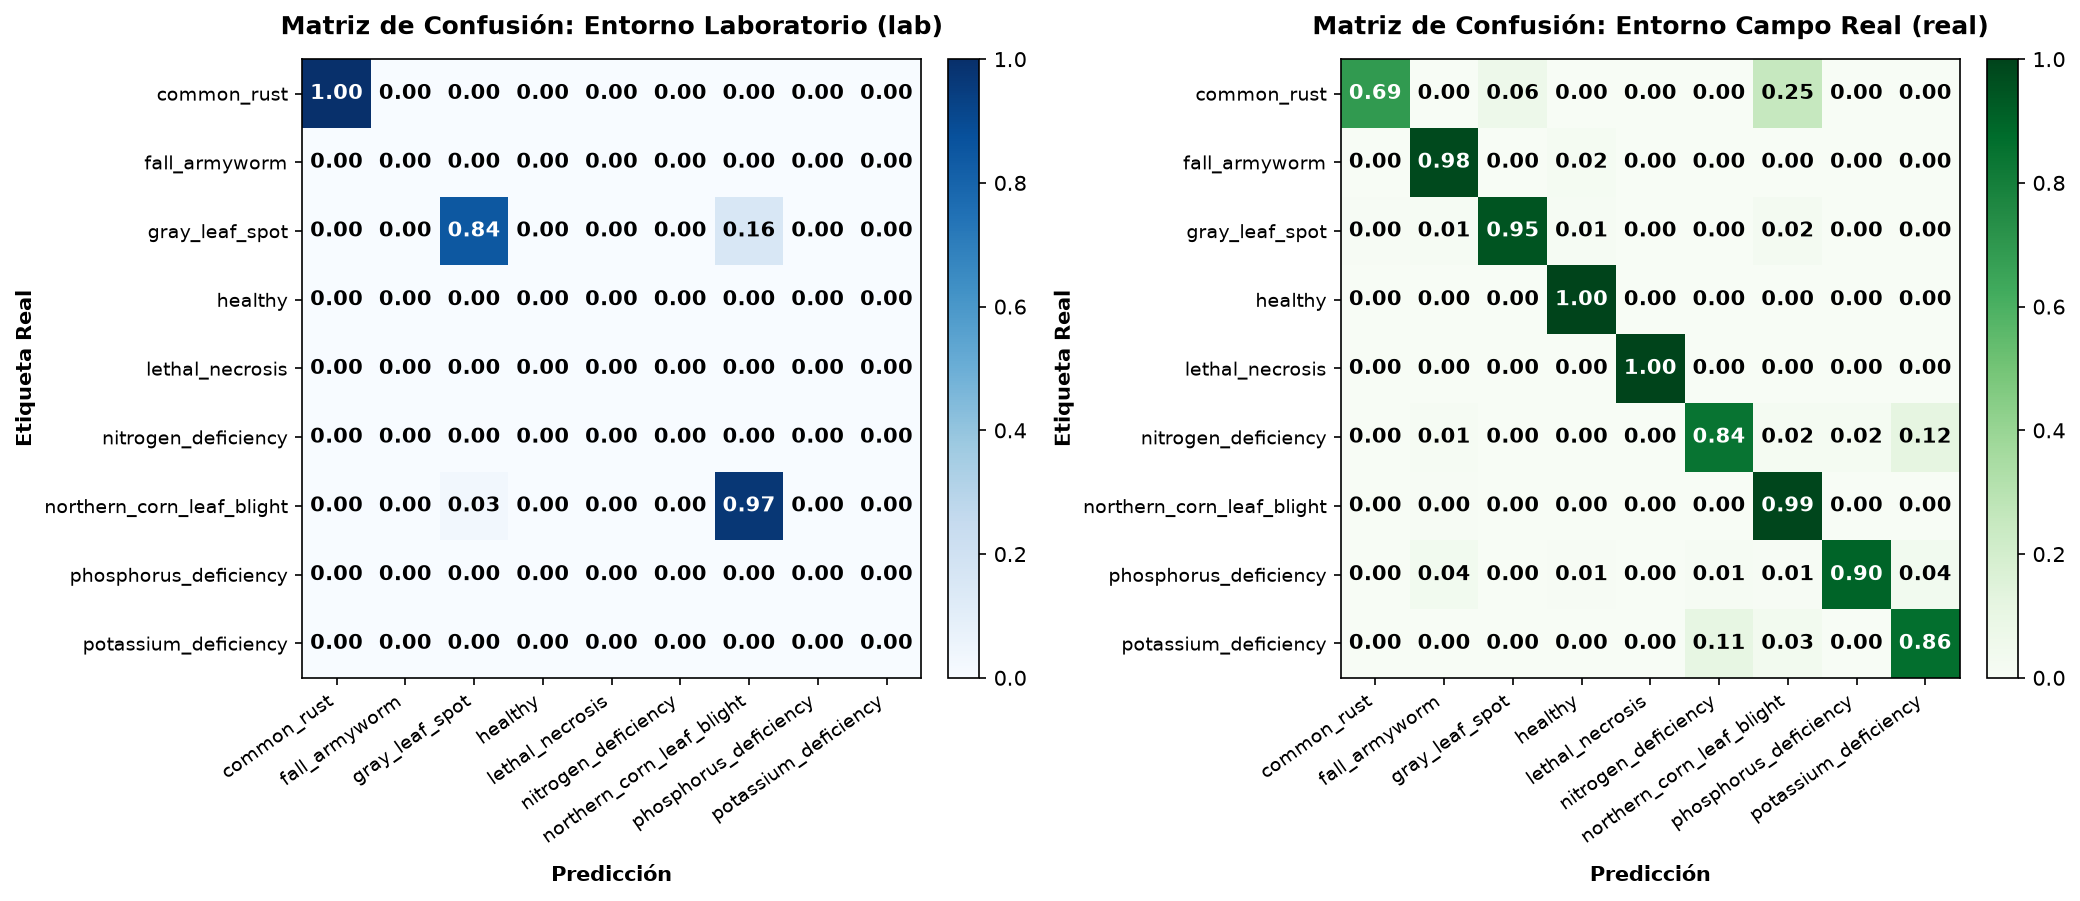
\includegraphics[width=\linewidth]{images/fairness/disaggregated_confusion_matrices.png}
\caption{Matrices desagregadas Lab vs. Campo.}
\label{fig:fairness_cm}
\end{minipage}
\caption{Auditor\'ia de equidad e imparcialidad entre condiciones fotogr\'aficas.}
\label{fig:fairness_panel}
\end{figure}

El an\'alisis granular de la tasa de falsos negativos ($FNR$) mostr\'o una asimetr\'ia relevante, aunque con muestras peque\~nas en campo (Tabla~\ref{tab:fnr_c3}):
\begin{itemize}
\item La \textbf{Roya Com\'un} es casi infalible en laboratorio ($FNR = 0.31\%$, 1 fallo en 322 casos) pero \textbf{falla en el 31.25\% de los casos en campo real} (5 fallos en 16 casos). Esto ocurre porque el 95\% del corpus hist\'orico de roya proviene de hojas recortadas sobre mesas de laboratorio.
\item La \textbf{Mancha Gris} exhibe el patr\'on inverso: $15.58\%$ de error en laboratorio frente a solo $5.16\%$ en campo aut\'entico.
\end{itemize}

\begin{table}[H]
\caption{Tasa de falsos negativos ($FNR$) desagregada por clase y entorno}
\label{tab:fnr_c3}
\centering
\small
\begin{singlespace}
\begin{tabular}{lcccc}
\toprule
\textbf{Patolog\'ia Evaluada} & \textbf{$FNR$ Laboratorio} & \textbf{Soporte ($N$)} & \textbf{$FNR$ Campo Real} & \textbf{Soporte ($N$)} \\
\midrule
Roya Com\'un & 0.31\% & 322 & \textbf{31.25\%} & 16 \\
Mancha Gris (GLS) & 15.58\% & 77 & 5.16\% & 213 \\
Tiz\'on Foliar (NCLB) & 3.01\% & 133 & 1.01\% & 892 \\
\bottomrule
\end{tabular}
\end{singlespace}
\end{table}

\subsection{Capacidades del diagn\'ostico: dependencia del fondo}

Para desentra\~nar si el modelo miraba la hoja o el entorno, se ejecut\'o una auditor\'ia de oclusi\'on espacial geom\'etrica sobre las 5~015 muestras de prueba frente a un predictor nulo constante (Tabla~\ref{tab:ablacion_c3} y Figura~\ref{fig:ablacion_grafico}).

\begin{table}[H]
\caption{Auditor\'ia de ablaci\'on espacial con control nulo en el conjunto de prueba}
\label{tab:ablacion_c3}
\centering
\small
\begin{singlespace}
\begin{tabular}{lccccc}
\toprule
\textbf{Condici\'on de Entrada} & \textbf{Regi\'on Visible} & \textbf{\'Area (\%)} & \textbf{Exactitud} & \textbf{Exceso s/Nulo} & \textbf{Conf. Retenida} \\
\midrule
Imagen original completa & Toda la escena & 100.0\% & 97.91\% & +71.77 pp & 100.0\% \\
\textbf{Oclusi\'on central} & \textbf{Anillo perif\'erico} & \textbf{63.7\%} & \textbf{79.46\%} & \textbf{+53.32 pp} & \textbf{69.16\%} \\
Oclusi\'on perif\'erica & Caja central & 36.3\% & 42.25\% & +16.11 pp & 42.66\% \\
Control nulo (sin p\'ixeles) & Clase mayoritaria & 0.0\% & 26.14\% & 0.0 pp & — \\
\bottomrule
\end{tabular}
\end{singlespace}
\end{table}

\begin{figure}[H]
\centering
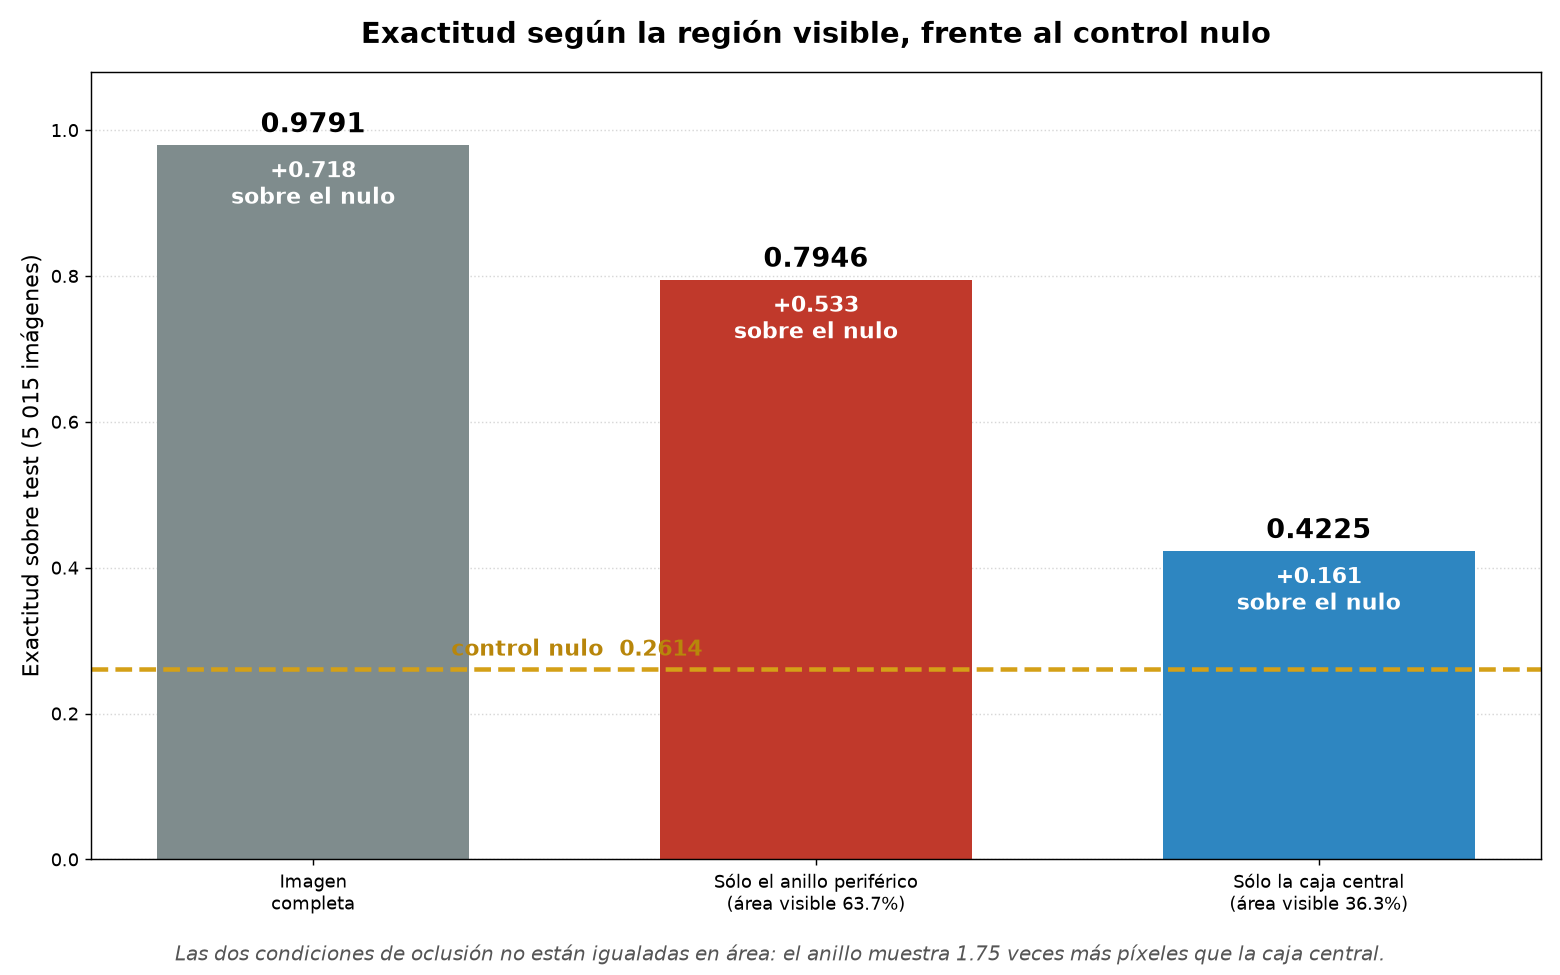
\includegraphics[width=0.62\linewidth]{images/resultados/ablacion_control_nulo.png}
\caption{Exactitud seg\'un la regi\'on geom\'etrica visible frente al azar nulo.}
\label{fig:ablacion_grafico}
\end{figure}

Al ocluir la regi\'on central de la imagen (36.3\% del \'area), el clasificador conserva un \textbf{79.46\% de exactitud}; esta sensibilidad se mantiene dentro de los m\'argenes esperados seg\'un el an\'alisis de equidad. En cambio, al ocluir la periferia, la exactitud cae a 42.25\% y el an\'alisis marca dependencia cr\'itica de la regi\'on perif\'erica (riesgo CR\'ITICO, \texttt{shortcut\_confirmed}). Este hallazgo es consistente con que el fondo aporta se\~nal de clase, aunque el experimento no aisla causalmente la lesi\'on del fondo, por lo que la interpretaci\'on debe tomarse como hip\'otesis de trabajo que motiva el marco gu\'ia de captura.

\noindent\textbf{El fallo instructivo de la segmentaci\'on:} Intentar aislar la hoja forzando una m\'ascara negra autom\'atica con YOLO degrad\'o el Macro $F_1$ a \textbf{0.7191}. Esto demostr\'o que los errores de m\'ascara en hojas complejas destruyen tejido leg\'itimo y alteran la estad\'istica de color de la red convolucional.

\noindent\textbf{Interpretabilidad con Grad-CAM y SHAP:} Al evaluar mapas de calor locales (Figuras~\ref{fig:gradcam_panel_c3} y~\ref{fig:shap_lime_c3}), los m\'etodos de atribuci\'on destacan las lesiones visibles. Sin embargo, al medir el \textbf{exceso de atribuci\'on foliar} (fracci\'on sobre la hoja menos la cobertura de la m\'ascara), el exceso medio fue de apenas \textbf{+0.037}. La firma de fondo es un fen\'omeno difuso de baja frecuencia distribuido en miles de p\'ixeles que no satura los mapas locales pero gobierna la predicci\'on global.

\begin{figure}[H]
\centering
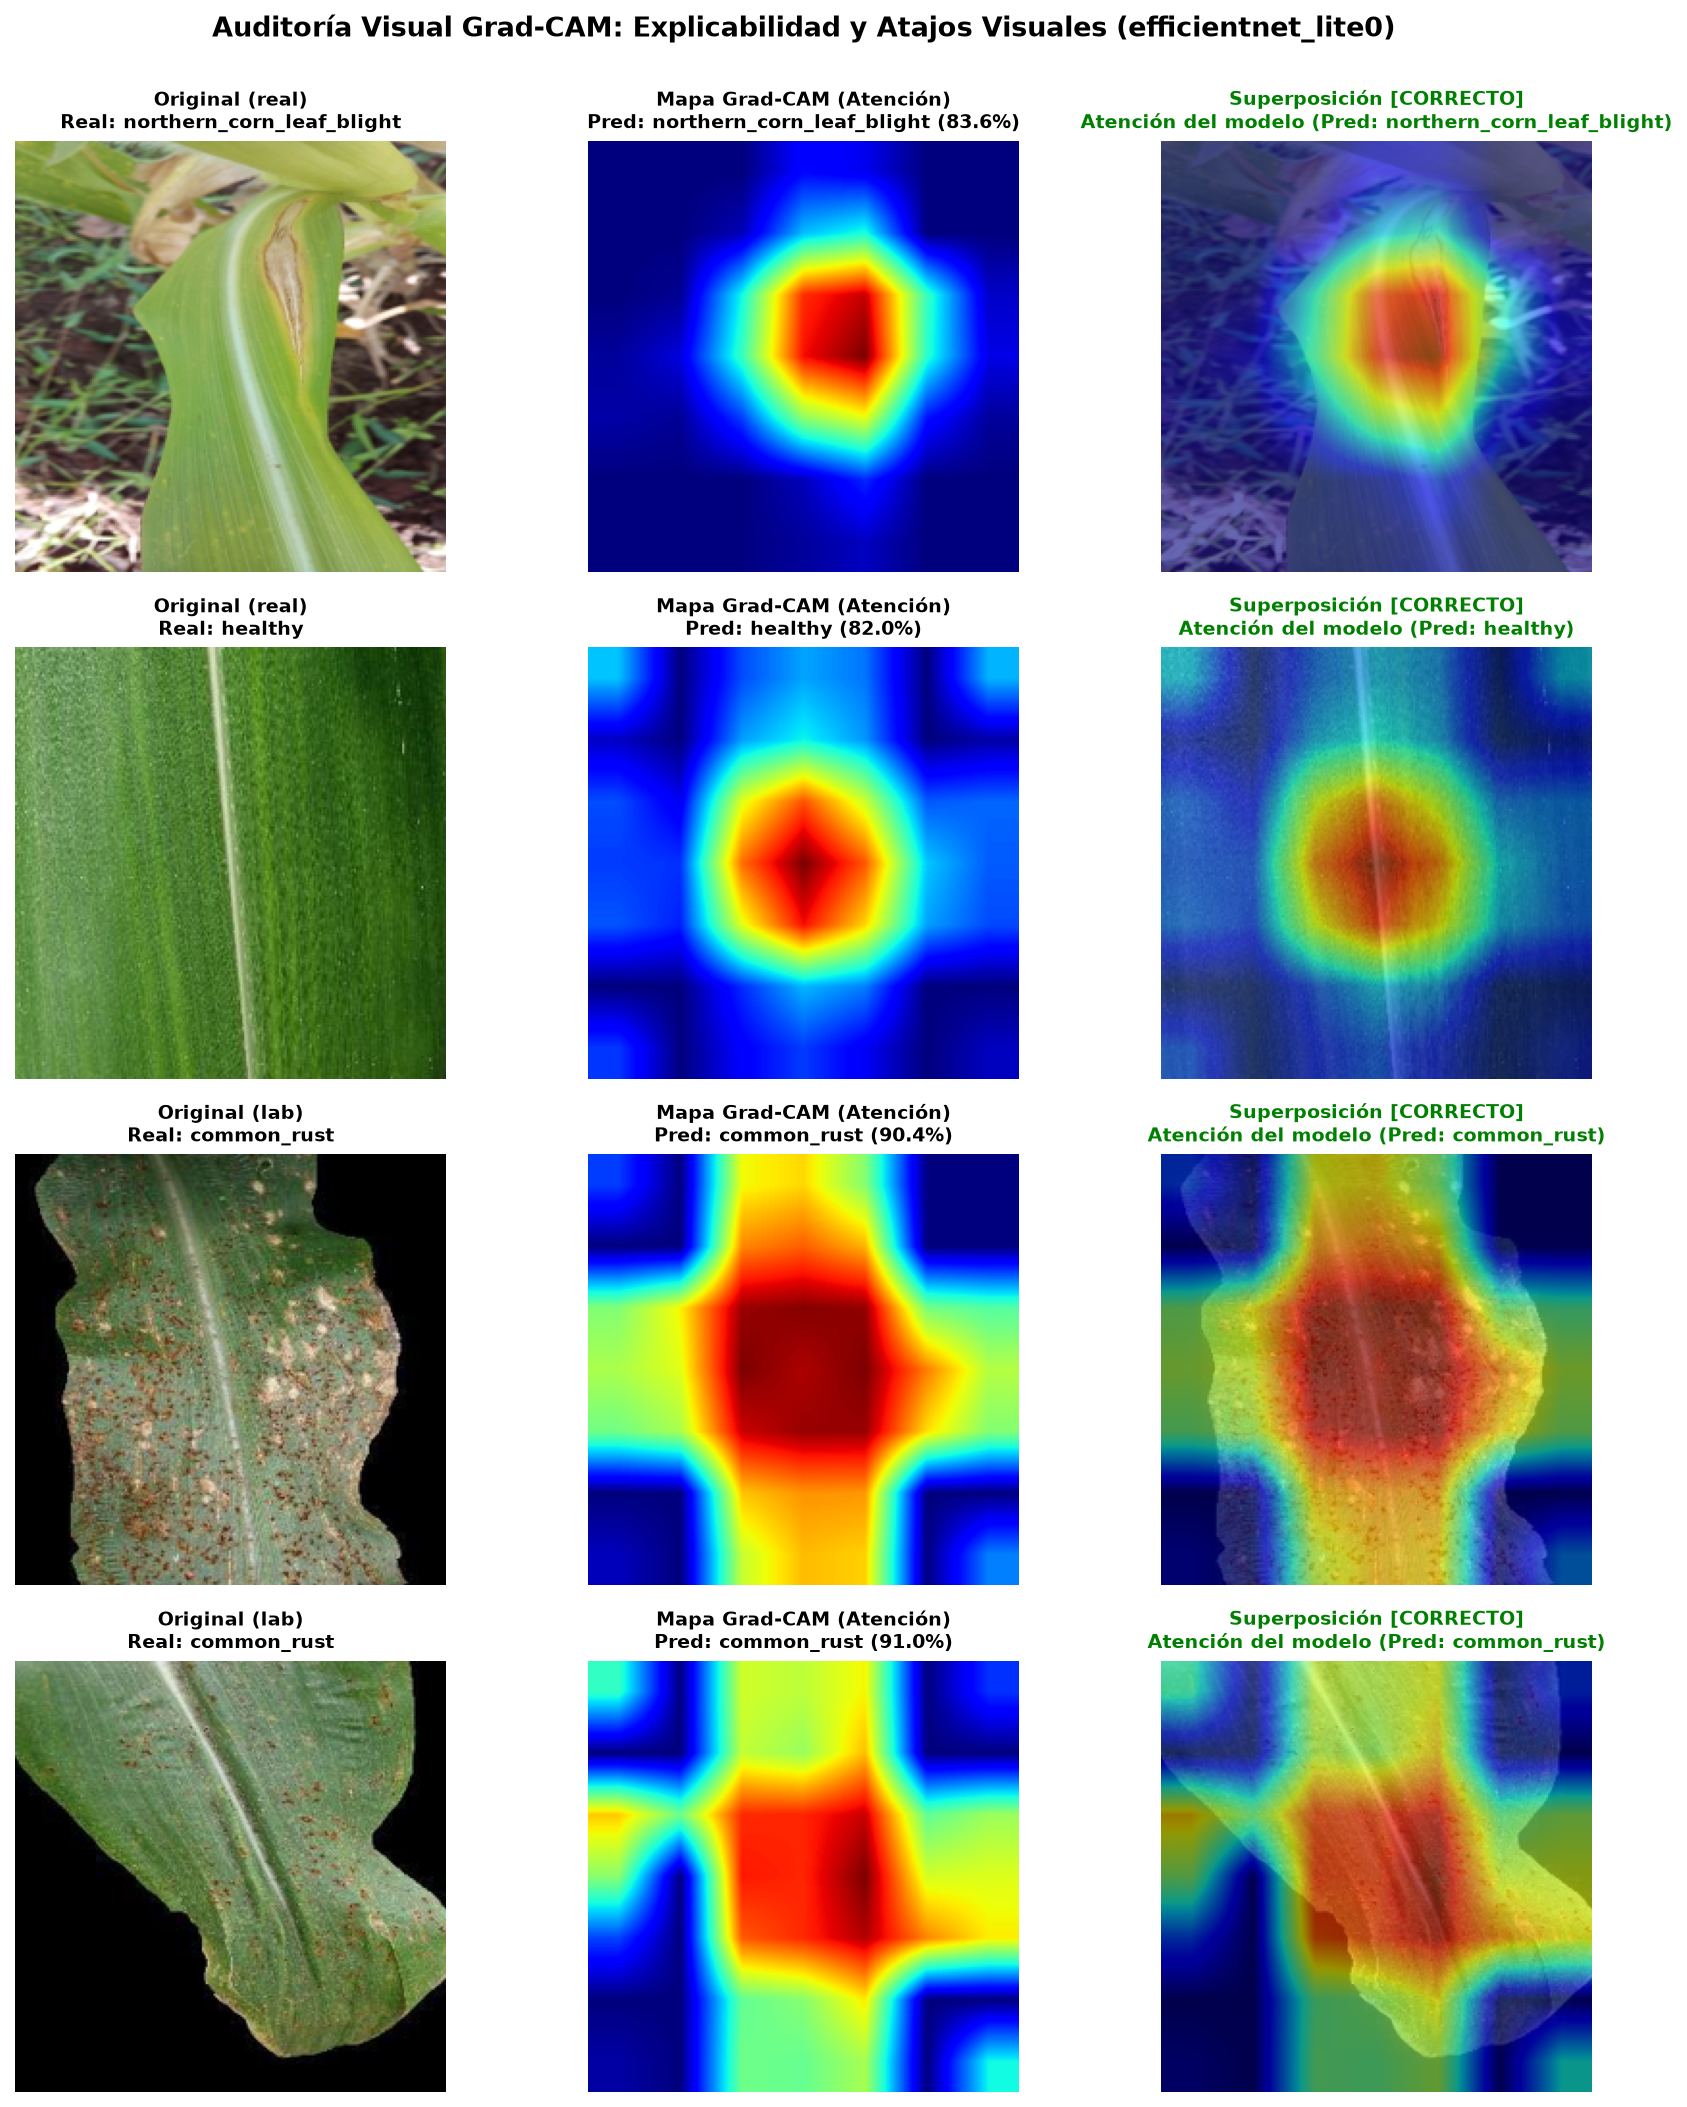
\includegraphics[width=0.72\linewidth]{images/fairness/gradcam_samples.png}
\caption{Mapas de activaci\'on Grad-CAM en muestras de campo real y laboratorio.}
\label{fig:gradcam_panel_c3}
\end{figure}

\begin{figure}[H]
\centering
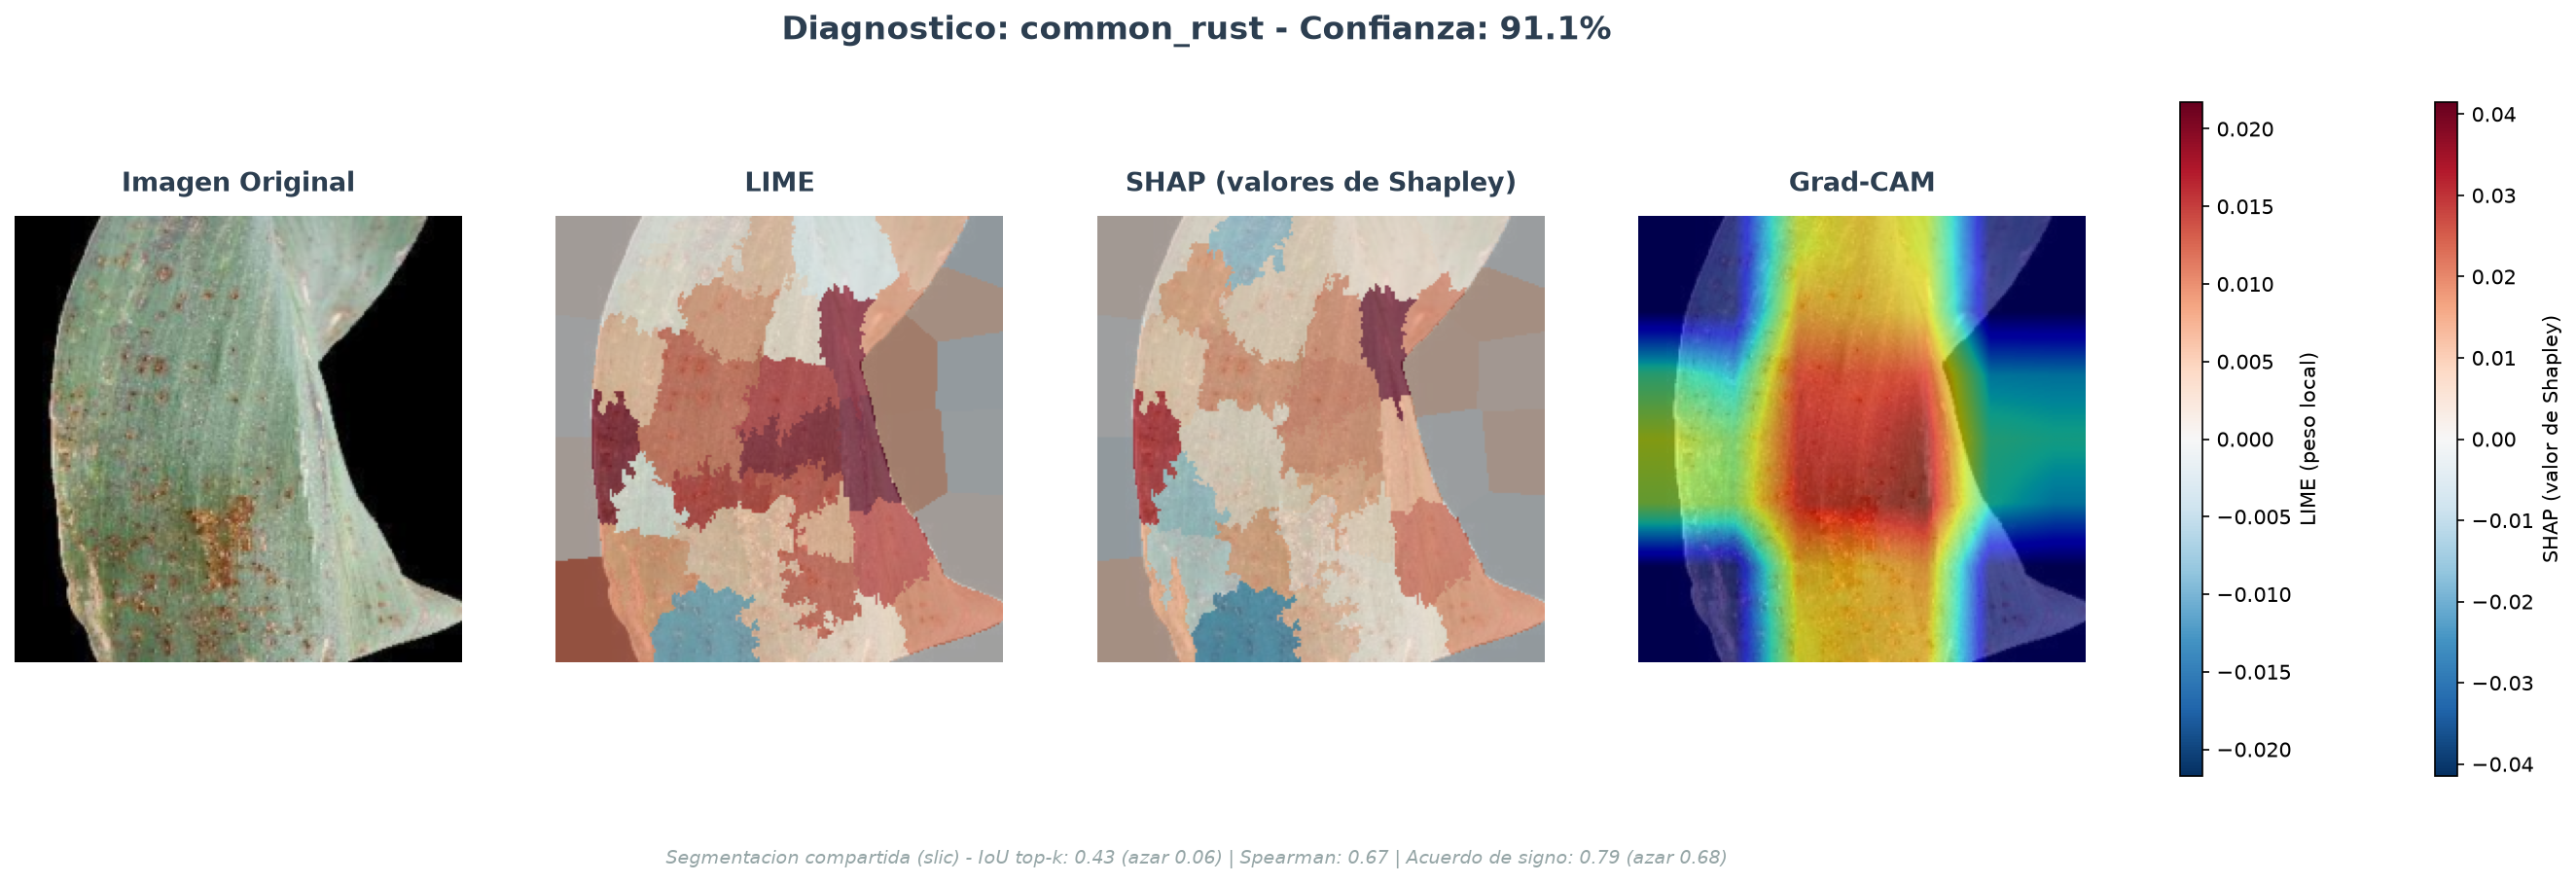
\includegraphics[width=0.65\linewidth]{images/xai/panel_compare_common_rust.png}
\caption{Panel comparado de explicabilidad local: LIME, SHAP y Grad-CAM.}
\label{fig:shap_lime_c3}
\end{figure}

\subsection{Soluci\'on integral: prototipo en hardware real}

El modelo \texttt{EfficientNet-Lite0} cuantizado a 8 bits (\textbf{Int8}) redujo su tama\~no hasta \textbf{3.56~MB} en el archivo desplegado en la aplicaci\'on, lo que representa una reducci\'on del 72\% frente a los 12.92~MB del modelo FP32 documentado en la exportaci\'on. La paridad num\'erica con el modelo FP32 se verific\'o sobre una muestra, y la retenci\'on de exactitud de la versi\'on cuantizada no se midi\'o sobre el conjunto de prueba completo.

Para validar el prototipo en condiciones de campo aut\'enticas, la aplicaci\'on m\'ovil nativa \textbf{DoctorMaiz} (desarrollada en React Native, TypeScript y motor \texttt{react-native-fast-tflite}) fue instalada y testeada en un smartphone f\'isico \textbf{Motorola edge 40 neo} (procesador MediaTek Dimensity 7030 octa-core a 2.5 GHz, 8~GB RAM, Android 15).

Las mediciones instrumentadas mediante \texttt{adb logcat} arrojaron latencias extraordinarias (Tabla~\ref{tab:latencias_movil_c3}):
\begin{itemize}
\item La inferencia pura en la CPU del tel\'efono requiri\'o una mediana de \textbf{60 milisegundos} (promedio 68 ms), frente a la meta de $\le 100$~ms para inferencia definida en la especificaci\'on.
\item El preprocesado bilineal tom\'o 41 ms.
\item El pipeline interactivo completo (captura, decodificaci\'on, inferencia, persistencia en SQLite y renderizado) tom\'o apenas \textbf{473 ms} en la mediana (\textit{Flujo Total}), frente a la meta de respuesta de 300~ms para el tiempo total definida en la especificaci\'on.
\item El consumo m\'aximo de memoria RAM se mantuvo por debajo de \textbf{85~MB}, garantizando fluidez en tel\'efonos b\'asicos.
\end{itemize}

\begin{table}[H]
\caption{Latencias operativas medidas en hardware f\'isico (Motorola edge 40 neo)}
\label{tab:latencias_movil_c3}
\centering
\small
\begin{singlespace}
\begin{tabular}{lccccp{4.8cm}}
\toprule
\textbf{Fase del Proceso} & \textbf{Mediana} & \textbf{Promedio} & \textbf{M\'inimo} & \textbf{M\'aximo} & \textbf{Acci\'on Operativa} \\
\midrule
Preprocesado & 41 ms & 157 ms & 19 ms & 675 ms & Decodificaci\'on y escalado bilineal. \\
\textbf{Inferencia Int8} & \textbf{60 ms} & \textbf{68 ms} & \textbf{34 ms} & \textbf{141 ms} & Evaluaci\'on TFLite en CPU con C++. \\
\textbf{Flujo Total} & \textbf{473 ms} & \textbf{548 ms} & \textbf{336 ms} & \textbf{977 ms} & Captura, c\'alculo OOD y UI final. \\
\bottomrule
\end{tabular}
\end{singlespace}
\end{table}

\noindent\textbf{Comprobaci\'on de la mitigaci\'on en la Interfaz de Usuario (UI/UX):} La aplicaci\'on solventa las limitaciones del modelo mediante un dise\~no ergon\'omico adaptado al productor (Figuras~\ref{fig:app_pantallas_1} y~\ref{fig:app_pantallas_2}):
\begin{enumerate}
\item \textbf{C\'amara con marco gu\'ia foliar (Figura~\ref{fig:app_cam_c3}):} Al instruir al agricultor a encuadrar la hoja y recortar autom\'aticamente el 24\% central de la escena (3.02 MP a partir del sensor de 12.6 MP), la app descarta el 75\% del fondo enga\~noso antes de inferir, neutralizando el sesgo de procedencia.
\item \textbf{Detector OOD de Mahalanobis (Figura~\ref{fig:app_ood_c3}):} Al apuntar a elementos extra\~nos (manos, suelo, ropa), la distancia multivariada supera el umbral 31.47 y el sistema despliega con prudencia: \textbf{«Imagen no reconocida»}.
\item \textbf{M\'odulo de contribuci\'on comunitaria (Figura~\ref{fig:app_contrib_c3}):} Permite almacenar fotos de milpas salvadore\~nas para subirlas cuando haya conectividad.
\item \textbf{Gu\'ias de severidad contextualizadas (Figura~\ref{fig:app_sev_c3}):} Ofrece al productor una escala gr\'afica de tres grados en lenguaje cotidiano con pautas de bioinsumos comerciales locales.
\end{enumerate}

\begin{figure}[H]
\centering
\begin{minipage}[b]{0.31\linewidth}
\centering
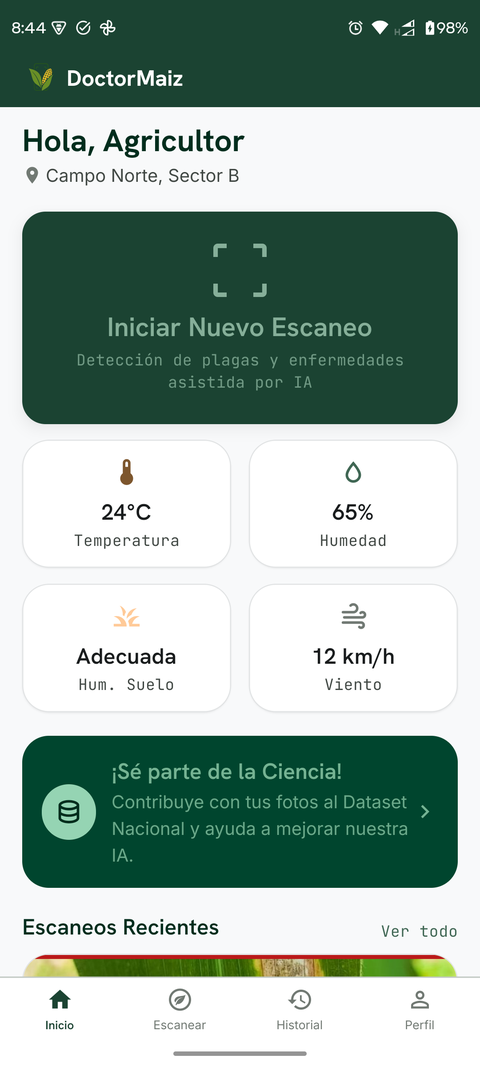
\includegraphics[width=\linewidth]{images/app/home.png}
\caption{Pantalla de inicio.}
\label{fig:app_home_c3}
\end{minipage}
\hfill
\begin{minipage}[b]{0.31\linewidth}
\centering
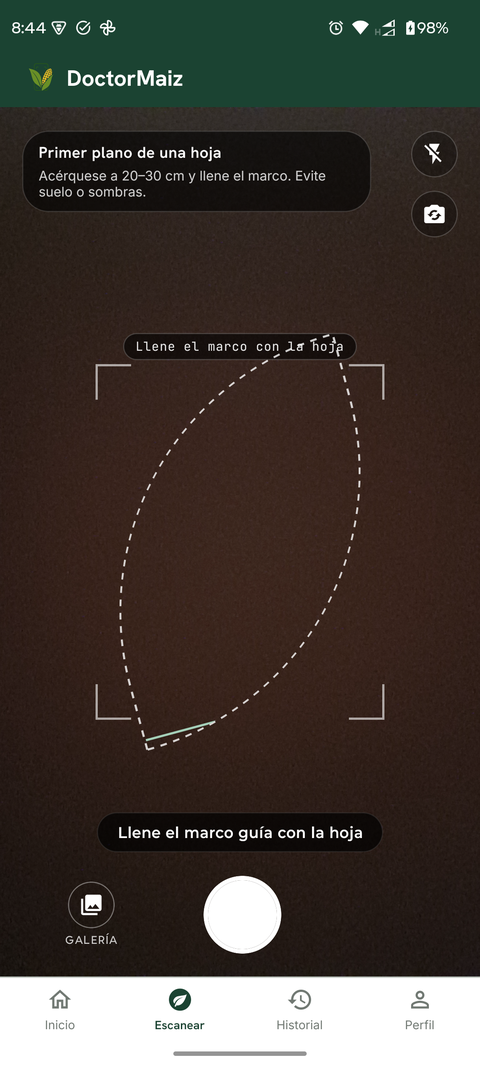
\includegraphics[width=\linewidth]{images/app/camara-marco-guia.png}
\caption{Marco gu\'ia foliar.}
\label{fig:app_cam_c3}
\end{minipage}
\hfill
\begin{minipage}[b]{0.31\linewidth}
\centering
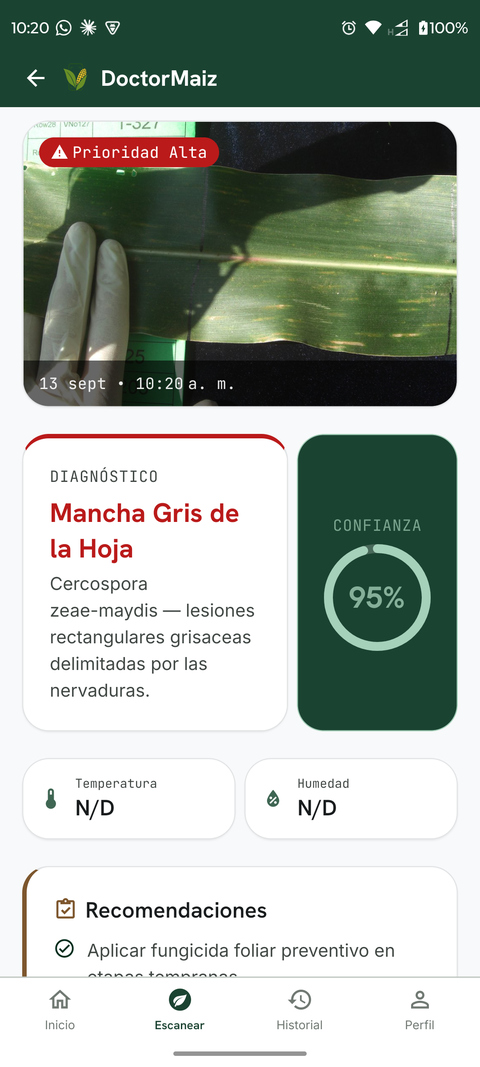
\includegraphics[width=\linewidth]{images/app/resultado-mancha-gris.png}
\caption{Diagn\'ostico obtenido.}
\label{fig:app_res_c3}
\end{minipage}
\caption{Flujo principal de la aplicaci\'on m\'ovil nativa DoctorMaiz.}
\label{fig:app_pantallas_1}
\end{figure}

\begin{figure}[H]
\centering
\begin{minipage}[b]{0.31\linewidth}
\centering
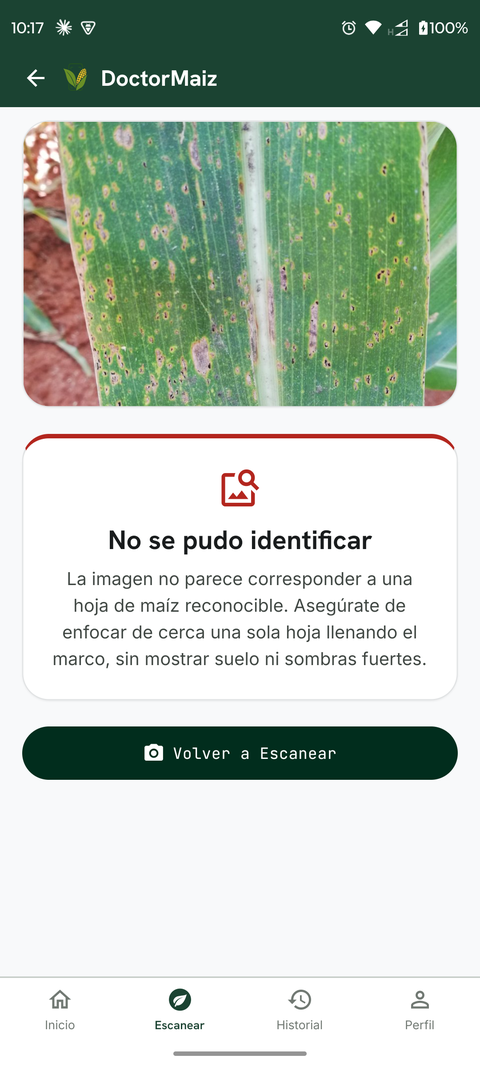
\includegraphics[width=\linewidth]{images/app/resultado-no-reconocida.png}
\caption{Bloqueo seguro por OOD.}
\label{fig:app_ood_c3}
\end{minipage}
\hfill
\begin{minipage}[b]{0.31\linewidth}
\centering
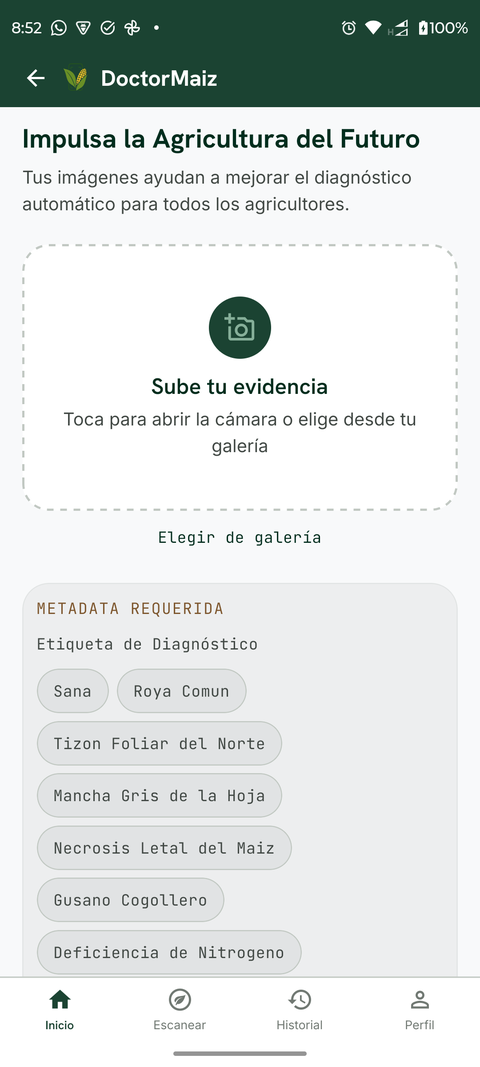
\includegraphics[width=\linewidth]{images/app/contribuir.png}
\caption{Aporte comunitario.}
\label{fig:app_contrib_c3}
\end{minipage}
\hfill
\begin{minipage}[b]{0.31\linewidth}
\centering
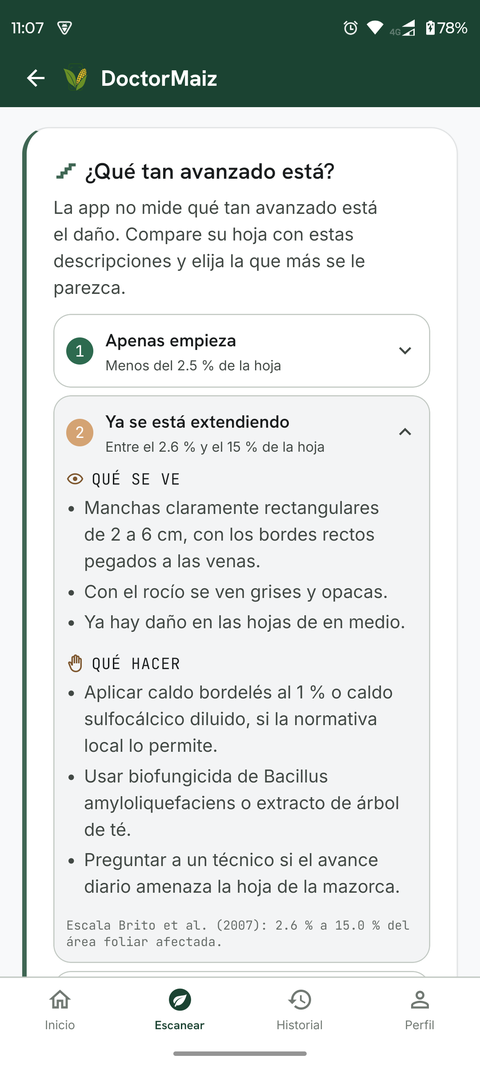
\includegraphics[width=\linewidth]{images/app/resultado-severidad.png}
\caption{Gu\'ia de severidad.}
\label{fig:app_sev_c3}
\end{minipage}
\caption{Mecanismos de seguridad, participaci\'on comunitaria y escalas agron\'omicas.}
\label{fig:app_pantallas_2}
\end{figure}

\section{Impacto Social y Recomendaciones de Pol\'itica P\'ublica}

El valor de esta investigaci\'on se consolida al traducir los avances matem\'aticos en cinco propuestas concretas dirigidas al Ministerio de Agricultura y Ganader\'ia (MAG) y al CENTA:

\begin{enumerate}
\item \textbf{Adopci\'on de DoctorMaiz como herramienta oficial de extensi\'on:} Homologar la app como asistente de bolsillo para los m\'as de 300 promotores del CENTA, estandarizando diagn\'osticos en caser\'ios remotos de Caba\~nas y Moraz\'an sin consumir datos celulares.
\item \textbf{Red Nacional de Alerta Fitosanitaria Temprana:} Alimentar un tablero epidemiol\'ogico centralizado en el MAG sincronizando an\'onimamente fechas y coordenadas de capturas cuando haya cobertura, activando cercos sanitarios ante rebrotes de necrosis letal.
\item \textbf{Banco Nacional Participativo de Datos Agr\'icolas:} Financiar brigadas fotogr\'aficas participativas junto a estudiantes de la Universidad de El Salvador para capturar variedades locales (h\'ibrido H-59 y criollos), cerrando definitivamente la brecha de dominio detectada.
\item \textbf{Campa\~nas comunitarias de alfabetizaci\'on digital agropecuaria:} Ense\~nar a cooperativas y ADESCOs el uso correcto del marco gu\'ia, posicionando la IA como aliada del saber campesino y no como sustituto.
\item \textbf{Soberan\'ia tecnol\'ogica y protecci\'on de datos campesinos:} Conservar el software bajo licencias de c\'odigo abierto (MIT/Apache 2.0), impidiendo la privatizaci\'on del patrimonio de datos agr\'icolas por transnacionales de semillas.
\end{enumerate}
